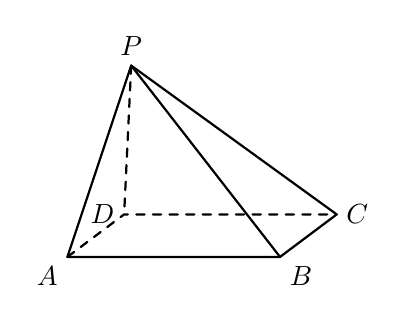
\begin{tikzpicture}[>=stealth,scale=0.9,line cap=round,line join=round]
  \coordinate (A) at (0,0);
  \coordinate (B) at (3,0);
  \coordinate (D) at (0.8,0.6);
  \coordinate (C) at (3.8,0.6);
  \coordinate (P) at (0.9,2.7);
  \draw[thick] (A)--(B)--(C)--(P)--cycle;
  \draw[thick] (P)--(B);
  \draw[thick,dashed] (A)--(D)--(C);
  \draw[thick,dashed] (P)--(D);
  \node[below left] at (A) {$A$};
  \node[below right] at (B) {$B$};
  \node[right] at (C) {$C$};
  \node[left] at (D) {$D$};
  \node[above] at (P) {$P$};
\end{tikzpicture}
